\documentclass[twocolumn,oneside,a4paper,12pt]{article}

% ---------------- Para Modificar ---------------- 
\newcommand{\principal}{Volumes}
\newcommand{\conteudo}{}
\newcommand{\turmas}{3~EMSI~A e do 3~EMSI~B}

\date{abril de 2021}

\newcommand{\citacao}{Que nada nos defina. Que nada nos sujeite. Que a liberdade seja a nossa própria substância.}
\newcommand{\autorcitacao}{Simone de Beauvoir}
% ------------------------------------------------

%-------------------------------------------------
\usepackage[english,brazilian]{babel}
\usepackage[alf]{abntex2cite}
\usepackage[utf8]{inputenc}
\usepackage[T1]{fontenc}
\usepackage[top=15mm, bottom=15mm, left=10mm, right=10mm]{geometry}
\usepackage{framed,booktabs,color,hyperref,graphicx}
\usepackage{amsfonts,amsthm,cancel}
\usepackage{subfigure,enumerate,float}
  
\definecolor{shadecolor}{rgb}{0.8,0.8,0.8}
\pagenumbering{arabic}

% Colunas
\usepackage{multicol}
\columnsep=10mm %Espaçamento entre colunas.
\setlength{\columnseprule}{1pt}

% Cabeçalho
\usepackage{fancyhdr}
\pagestyle{fancy}
\lhead{\textbf{\principal}}
\rhead{}
\renewcommand{\headrulewidth}{1pt} % espessura da linha do cabeçalho
\renewcommand{\footrulewidth}{1pt} % espessura da linha do rodapé

% Parágrafo
\setlength{\parindent}{1.25cm}

\newtheorem{problema}{Problema}
\newtheorem{exercicio}{exercicio}
\newtheorem{exemplo}{Exemplo}
\newtheorem{questao}{Questão}

\usepackage[skip=10pt]{caption}
\captionsetup{font={stretch=0.4,small}}

\newcommand{\FRASE}{\textit{``\citacao ''}\\(\textbf{\autorcitacao})}

\title{\LINHAHORIZONTAL \\\textbf{\\ \principal}\footnote{Resumo para os estudos das aulas não presenciais no período de quarentena para as turmas do \turmas .}\\\LINHAHORIZONTAL}

\newcommand{\LINHAHORIZONTAL}{\center \rule{16cm}{1.25pt}}
\newcommand{\sol}{\textbf{Solução}}

\newcommand{\m}[1]{\(\displaystyle {#1}\)}
\newcommand{\M}[1]{\[{#1}\]}

\author{\textbf{Professor Leandro Vieira}\\EREM Regina Pacis\\Palmeirina-PE}
\newcommand{\frase}{\begin{verse} \flushright{\FRASE} \end{verse}}


\begin{document}
\pagestyle{empty}
\cabecalho

\begin{enumerate}
\item Quantos anagramas existem da palavra FLOR?

\item Quantos anagramas possui a palavra FUTEBOL?

\item Oito pessoas vão se organizar lado a lado para tirar uma foto. De quantas maneiras distintas essas pessoas podem se organizar?

\item Quantos anagramas da palavra MOLECA não começam pela letra M?

\item Quantos anagramas da palavra CELULAR, possui as letras L, A, R juntas em qualquer ordem?

\item  Quantas palavras distintas podemos formar com a palavra PERNAMBUCO? Quantas começam com a sílaba PER?

\item Quantos anagramas da palavra PASTEL começam e terminam por consoante?

\item Os resultados do último sorteio da Mega-Sena foram os números 04, 10, 26, 37, 47 e 57. De quantas maneiras distintas pode ter ocorrido essa sequência de resultados?

\item Na palavra NORTE, quantos anagramas podem ser formados? Quantos começam com vogal?

\item Tomando como base a palavra UFPEL, resolva as questões a seguir.
\begin{enumerate}
    \item Quantos anagramas podem ser formados de modo que as vogais estejam sempre juntas?
    \item Quantos anagramas podem ser formados com as letras UF juntas?
    \item Quantos anagramas podem ser formados com as letras PEL juntas e nessa ordem?
\end{enumerate}

\item Determine o número de anagramas que podem ser formados com as letras do nome ALEMANHA.

\item Utilizando o nome COPACABANA, calcule o número de anagramas formados desconsiderando aqueles em que ocorrem repetições consecutivas de letras.

\item Ao preencher um cartão da loteria esportiva, André optou pelas seguintes marcações: 4 coluna um, 6 coluna do meio e 3 coluna dois. De quantas maneiras distintas André poderá marcar os cartões? 

\item Em um torneio de futsal um time obteve 8 vitórias, 5 empates e 2 derrotas, nas 15 partidas disputadas. De quantas maneiras distintas esses resultados podem ter ocorrido?

\item Em uma prova composta de 20 questões envolvendo V ou F, de quantas maneiras distintas teremos doze respostas V e oito respostas F? 

\item A malha a seguir representa as ruas de um bairro. A e B são dos locais nesse bairro.

	\begin{figure}[!tbh]
	\center
	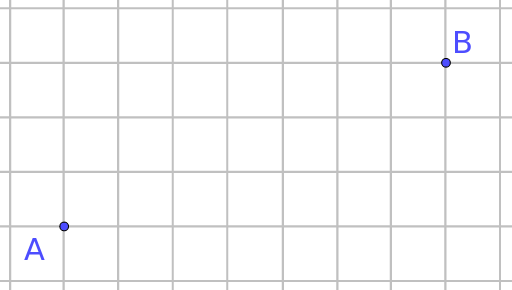
\includegraphics[width=8cm]{00}
	\end{figure}

\noindent De quantas formas é possível ir de A até B, tomando o menor caminho possível pelas ruas.
	
\item De quantas maneiras é possível ligar os pontos A e B 

	\begin{figure}[!tbh]
	\center
	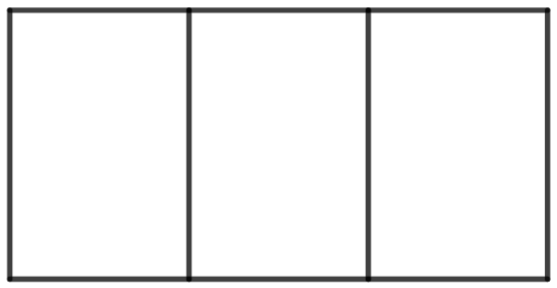
\includegraphics[width=8cm]{02}
	\end{figure}

\item

	\begin{figure}[!tbh]
	\center
	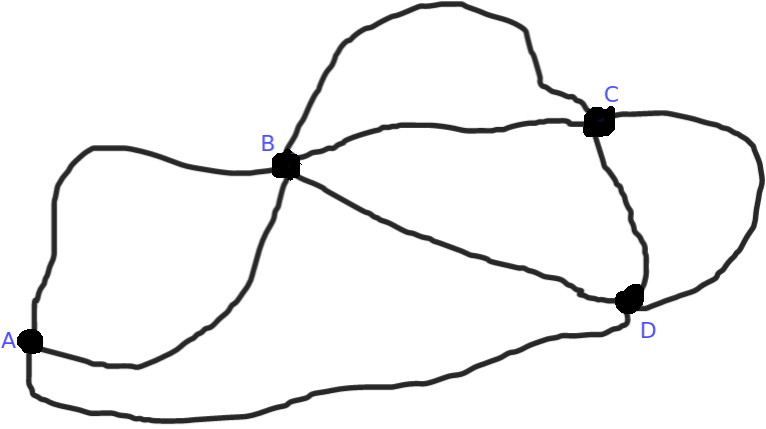
\includegraphics[width=8cm]{03}
	\end{figure}

\item

	\begin{figure}[!tbh]
	\center
	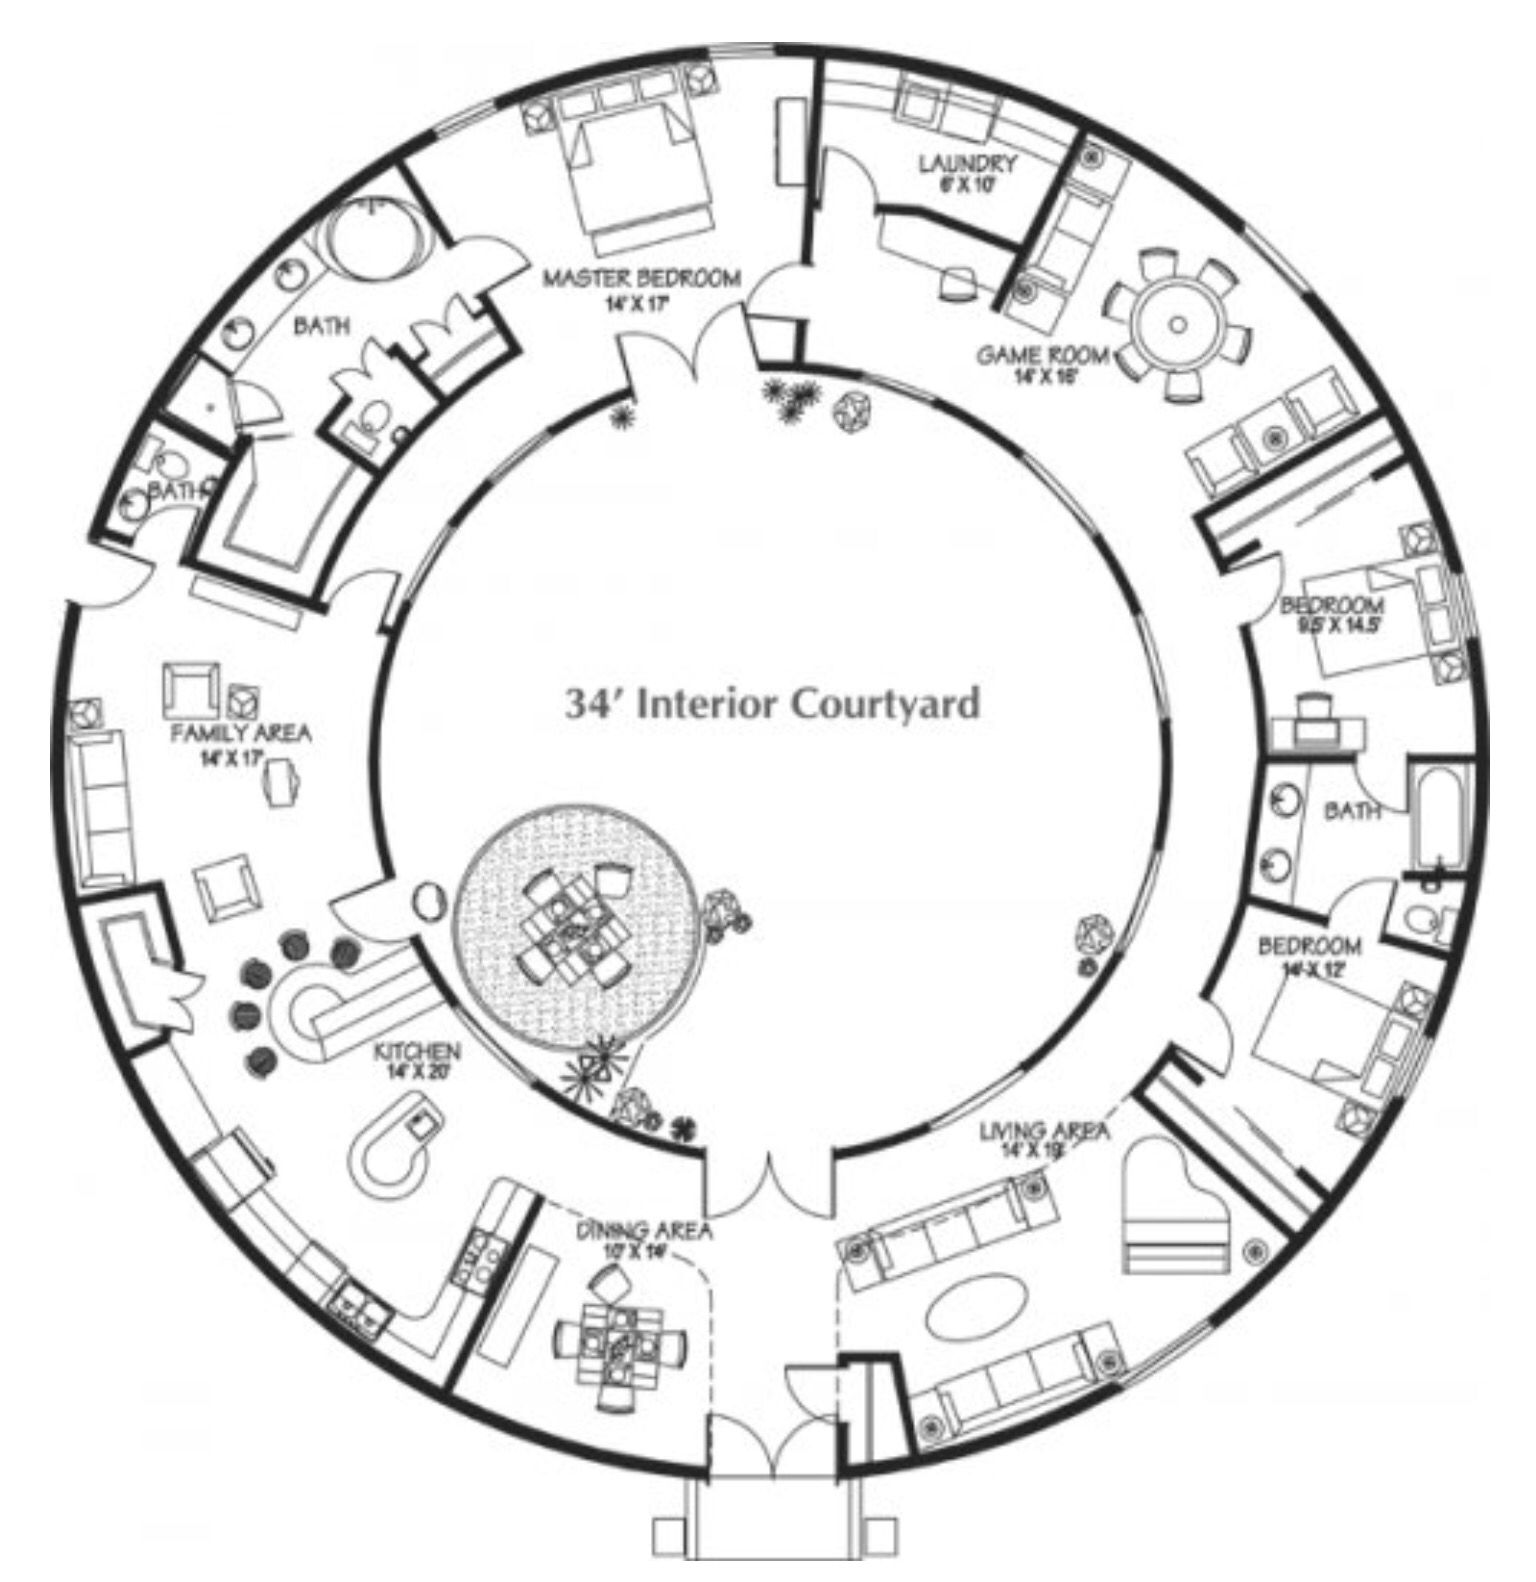
\includegraphics[width=8cm]{04}
	\end{figure}
	
\item

	\begin{figure}[!tbh]
	\center
	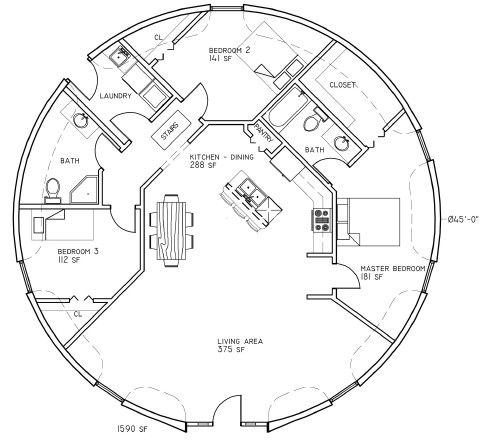
\includegraphics[width=8cm]{05}
	\end{figure}


\item

	\begin{figure}[!tbh]
	\center
	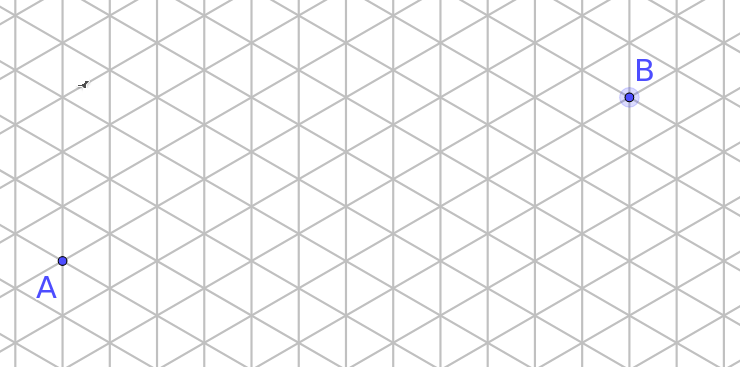
\includegraphics[width=8cm]{06}
	\end{figure}
	

\item

	\begin{figure}[!tbh]
	\center
	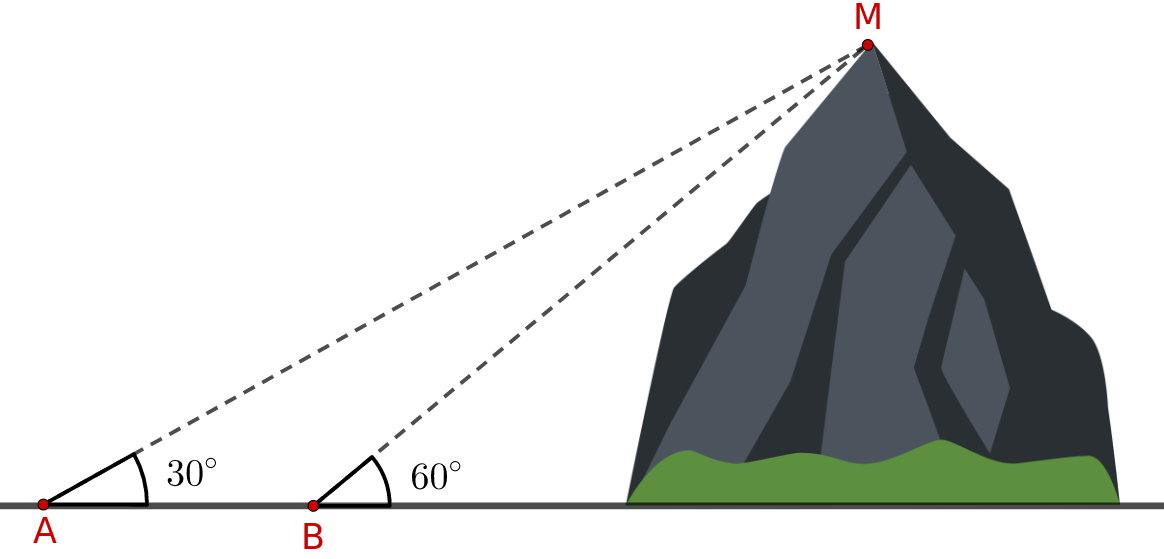
\includegraphics[width=8cm]{07}
	\end{figure}

\item

	\begin{figure}[!tbh]
	\center
	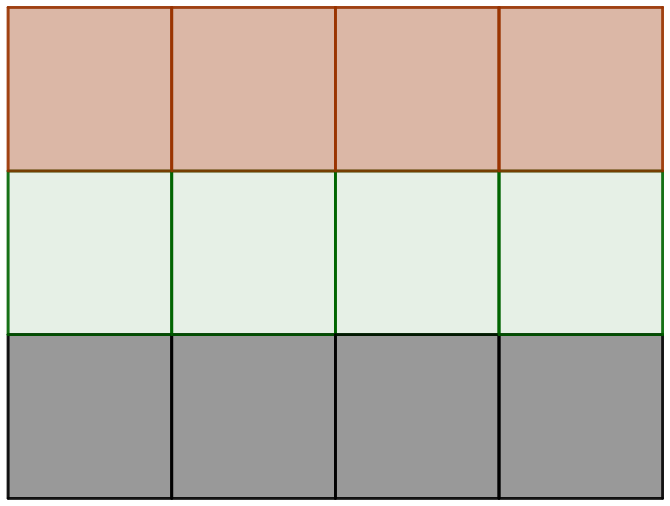
\includegraphics[width=8cm]{08}
	\end{figure}


\item O número de anagramas da palavra BIOCIÊNCIAS que terminam com as letras AS, nesta ordem é:
\begin{enumerate}
\item $9!$
\item $11!$
\item $9!/(3! \times 2!)$
\item $11!/2!$
\item $11!/3!$
\end{enumerate}

\item A figura a seguir representa parte do mapa de uma cidade onde estão assinalados as casas de João(A), de Maria(B), a escola(C) e um possível caminho que João percorre para, passando pela casa de Maria, chegar à escola. Qual o número total de caminhos distintos que João poderá percorrer, caminhando somente para o Norte ou Leste, para ir de sua casa à escola, passando pela casa de Maria?

	\begin{figure}[!tbh]
	\center
	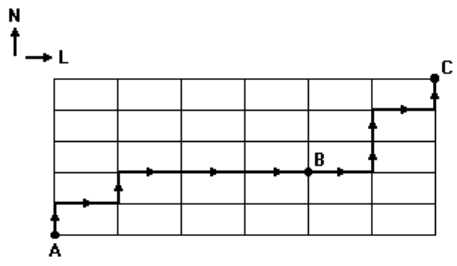
\includegraphics[width=8cm]{22}
	\end{figure}

\item Seis pessoas, entre elas João e Pedro, vão ao cinema. Existem seis lugares vagos, alinhados e consecutivos. O número de maneiras distintas como as seis podem sentar-se sem que João e Pedro fiquem juntos é
\begin{enumerate}
\item 720
\item 600
\item 480
\item 240
\item 120
\end{enumerate}

\item No desenho a seguir, as linhas horizontais e verticais representam ruas, e os quadrados representam quarteirões. A quantidade de trajetos de comprimento mínimo ligando A e B que  passam por C é

	\begin{figure}[!tbh]
	\center
	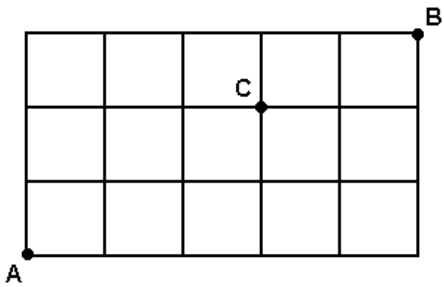
\includegraphics[width=8cm]{21}
	\end{figure}

\begin{enumerate}
\item 12
\item 13
\item 15
\item 24
\item 30
\end{enumerate}

\item +Uma pessoa quer comprar 6 pastéis em uma lanchonete. Há pastéis de camarão, frango, carne e queijo. Sabendo-se que podem ser compradas de zero a seis pastéis de cada tipo, de quantas maneiras diferentes esta compra pode ser feita?

\begin{enumerate}
\item 12
\item 13
\item 15
\item 24
\item 30
\end{enumerate}

\end{enumerate}

\FRASE
\end{document}
